\section{Boundary First Flattening}
In this section, I will get into details of my project on boundary first flattening. The algorithm is based on differential geometry. This section is organized as follows: I will first introduce the theoretical background. Then I will give details on my implementation.

\subsection{Theoretical Background}

\subsubsection{Conformal Maps}
In complex analysis,  conformal maps are equivlent to holomorphic maps, that is, the differentials of these map satisfy Cauchy-Riemann equation:
\begin{equation}
\frac{\partial f}{\partial \bar{z}} = 0
\end{equation}

One important property is that all comformal maps are harmonic maps, that is, 
\begin{equation}
\Delta f = 0
\end{equation}
But the reverse direction is not true.

\subsubsection{Poisson Problems}
Poisson problem is stated as follows:

Dirichlet-type condition:
\begin{equation}
\begin{split}
\Delta a &= \phi \ \ \ & on\  M\\
a &= g , & on\ \partial M
\end{split}
\end{equation}
Or Riemann-type condition:
\begin{equation}
\begin{split}
\Delta a &= \phi \ \ \ & on\  M\\
\frac{\partial a}{\partial n} &= h , & on\ \partial M 
\end{split}
\end{equation}

We will use discrete Poisson equation on a mesn $M$:

\begin{equation}
\left[\begin{matrix}
A_{II} & A_{IB}\\
A_{BI} & A_{BB}
\end{matrix}\right] \left[\begin{matrix}
a_I\\
a_B
\end{matrix}\right]
= \left[\begin{matrix}
\phi_I\\
\phi_B - h\end{matrix}\right]
\label{eq:relation}
\end{equation}

where $M$ is the cotangent Laplacian matrix.

Known $A$, Dirichlet-type conditions and Riemann-type conditions can be converted to each other: Given $h$, we simply solve the Poisson equation and set 
\begin{equation}
g = \Lambda^*_\phi h = a_B,
\end{equation}
Given $g$, we can convert it to $h$  by
\begin{equation}
h = \Lambda_\phi g = \phi_B - A_{IB}^TA_{II}^{-1}(\phi_I - A_{IB}g) - A_{BB}g
\end{equation}


\subsubsection{Cherrier Formula}
Cherrier formula \cite{CHERRIER1984154} is the core fact which induces the BFF algorithm. 

For a conformal map $f: M \rightarrow \tilde{M}$, we have 
\begin{equation}
\begin{split}
\Delta u = K - e^{2u} \tilde{K} \ \ \ &on\ &M\,\\
\frac{\partial u}{\partial n} = k - e^{u}\tilde{k} \ \ \ &on\     &\partial M
\end{split}
\end{equation}
where $u$ is conformal factor, $K$,$\tilde{K}$ are Gauss curvature of the source surface and  the target surface, $k, \tilde{k}$ is geodesic curvature of the source surface and the target surface.


The discrete version is the root of the algorithm:
\begin{equation}
\begin{split}
Au &=   \Omega - \tilde\Omega\  &on\  Int\  M\\
h &= k - \tilde{k}\ \  &on\ \partial M 
\end{split}
\label{eq:poisson}
\end{equation}
where $\Omega_i = 2\pi - \sum_{ijk \in F}\theta_i^{jk}$ defined on interior vertices, $k_i = \pi - \sum_{ijk \in F}\theta_i^{jk}$ defined on boundary vertices, which is the exterior angle at $v_i$. Note that $\Omega$ is defined to be zero at boundary vertices.



\section{Algorithm}

The pipeline of the BFF algorithm is as follows:

1) If boundray conformal factor ${u}$ is known, we compute bounadry target $k$ by: $$ \tilde{k} = k -\Lambda_{\Omega} u.$$
If target boundary $\tilde{k}$ is known, we compute boundary conformal factor $u$ by:: $$u = \Lambda_{\Omega}^{*}(k - \tilde{k}).$$

2) Define new boundary edge lengths as:
$$l_{ij}^* = e^{\frac{u_i + u_j}{2}}l_{ij}.$$ With $\tilde{k}$, which is exterior angles, we can integrate these two data into a closed loop.

3) Extend the loop into interior conformally.


\subsection{Loop Integration}
In step 2, usually, directly integrating $\tilde{k}$ over $l_{ij}^*$ won't give a closed loop, we should change edge length a little. So we solve the following quadratic optimization problem:

\begin{equation}
\begin{split}
&\min_{\tilde{l}}\ \  ||\tilde{l} - l^*||^2_2\\
s.t. & \sum_{ij\in \partial M} \tilde{l}_ij \tilde{T}_{ij}
\end{split}
\end{equation}

Here, $\tilde{T}_{ij}$ is the tangent vector of edge $ij$. We use the following procedure to compute tangent vectors:

1) Assume boundary vertex list is $\{0,1,2,3,...,|l|-1\}$. Compute cumulative angle as $$\phi_k = \sum_{i = 0}^{k-1}k_i.$$

2) Define tangent vectors as $$\tilde{T}_{ij} = (\cos {\phi_i}, \sin {\phi_j}).$$

\subsection{Conformal Interpolation}
In step 3, we need to get interior coordinates from fixed boundary data.

We know that all conformal maps are harmonic maps. So if the boundary data is truely from a conformal map, we can get this conformal map using the solver for harmonic maps. So the first method is using harmonic mapping directly. \textbf{Harmonic system} is Eq.\ref{eq:tutte} with cotangent weights.
But since we've changed the boundary lengths, conformality may not well preserved. 

Another method is to only use harmonic mapping on one component, and try to minimize conformal energy on the other component. This is done by Hilbert transform, which is defined by:
\begin{equation}
(\mathit{H}a_B)_j = \frac{1}{2}(a_k - a_i)
\end{equation}
where $i,j,k$ are three consecutive vertices on the boundary.

Then we use $\mathit{H}a_B$ as boundary data to solve the harmonic system. The solution is the other component. 
The shortcoming for this method is that the boundary exterior angles can not be well preserved.

\subsection{Experiments}
\subsubsection{Free Boundary Conformal Map}
Free boundary means preserving the boundary metric. We achieve this by setting conformal factors $u = 0$ on the boundary and using Hilbert transform to achieve interpolation. One example is shown in Fig. \ref{fig:boundary-free}.

\begin{figure}
\centering
\begin{subfigure}{0.3\textwidth}
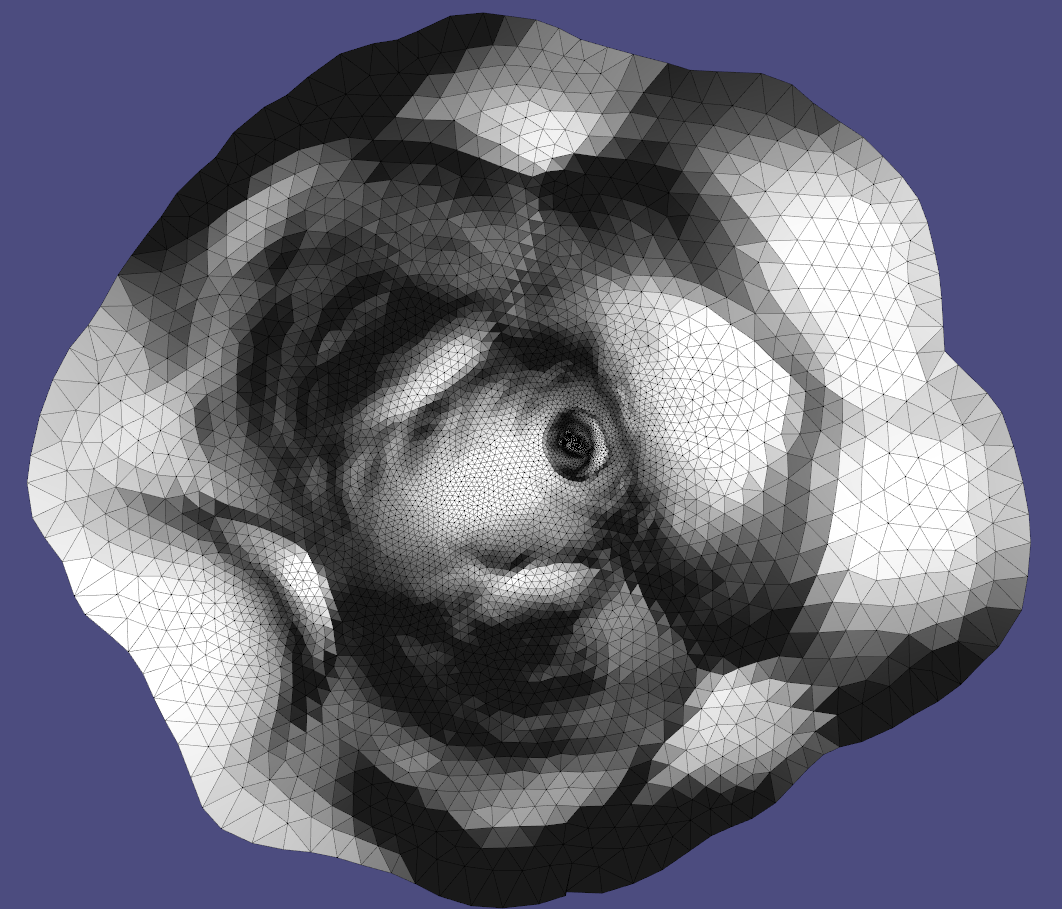
\includegraphics[height = \textwidth]{images/bunny_free_emb}
\caption{}
\end{subfigure}\ \ \ \ \ \ \ \ \ \ \ \ \
\begin{subfigure}{0.3\textwidth}
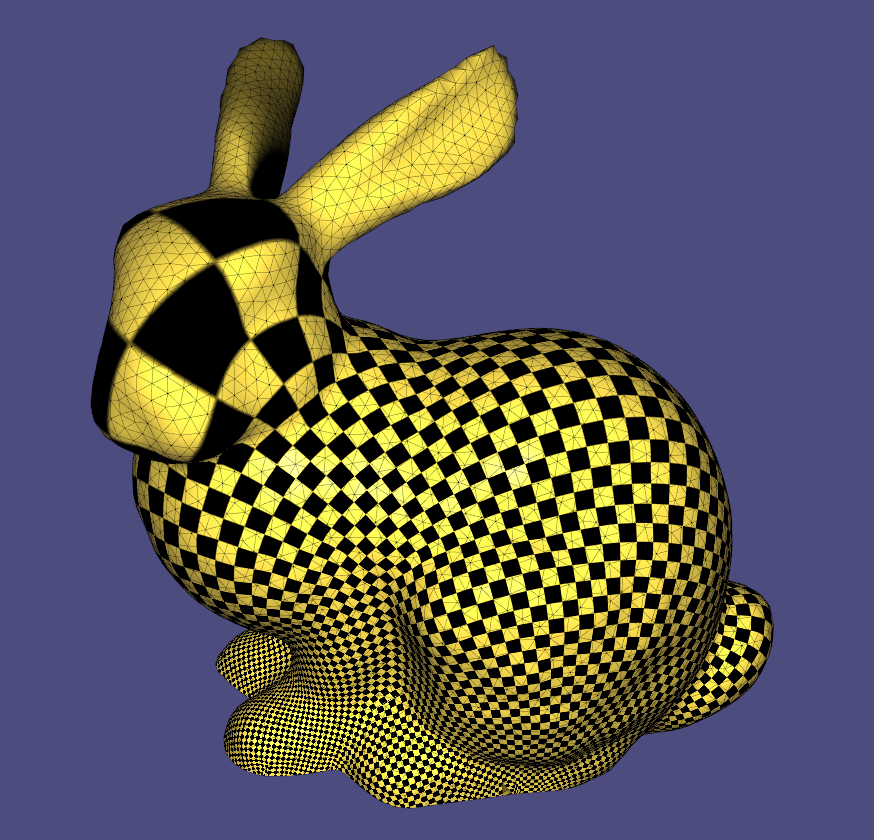
\includegraphics[height = \textwidth]{images/bunny_free_texture}
\caption{}
\end{subfigure}
\caption{Boundary free conformal map on bunny. (a) Embedding. (b) Texture mapping.}
\label{fig:boundary-free}
\end{figure}

\subsubsection{Polygonal-Boundary Conformal Map}
If we set some exterior angles be non-zero, and others be zero, the boundary will be a polygon. To precisely preseve boundary exterior angles, we should use harmonic interpolation. Some results are showned in Fig.\ref{fig:polygon}

\begin{figure}
\centering
\begin{subfigure}{0.25\textwidth}
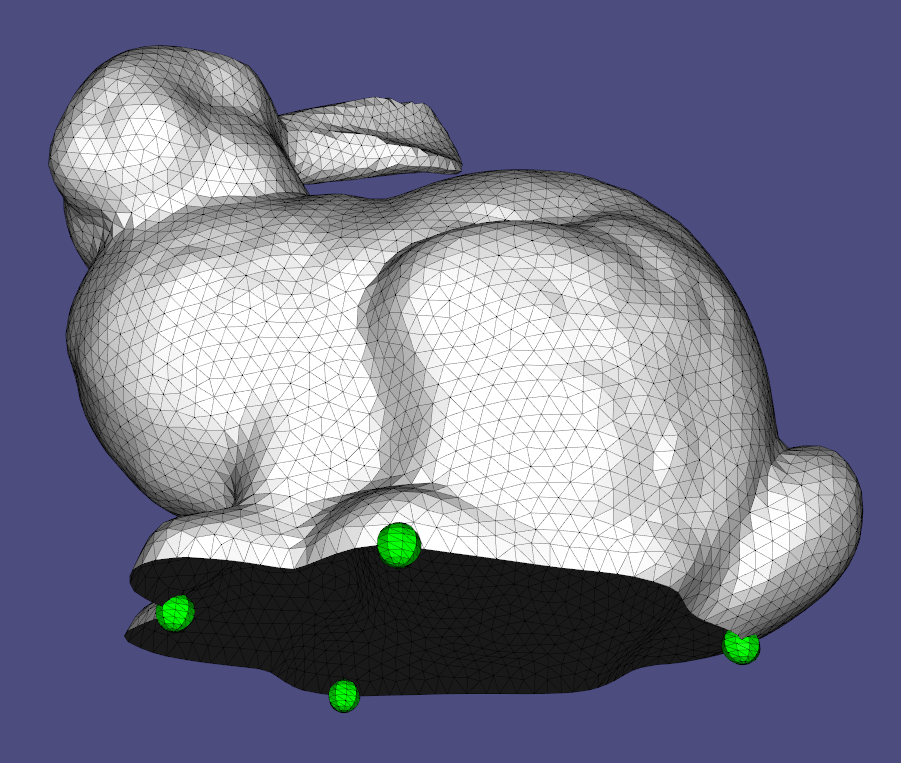
\includegraphics[height = \textwidth]{images/bunny_polygon}
\caption{}
\end{subfigure}\ \ \ \ \ \ \ \ \ \ \ \ \
\begin{subfigure}{0.25\textwidth}
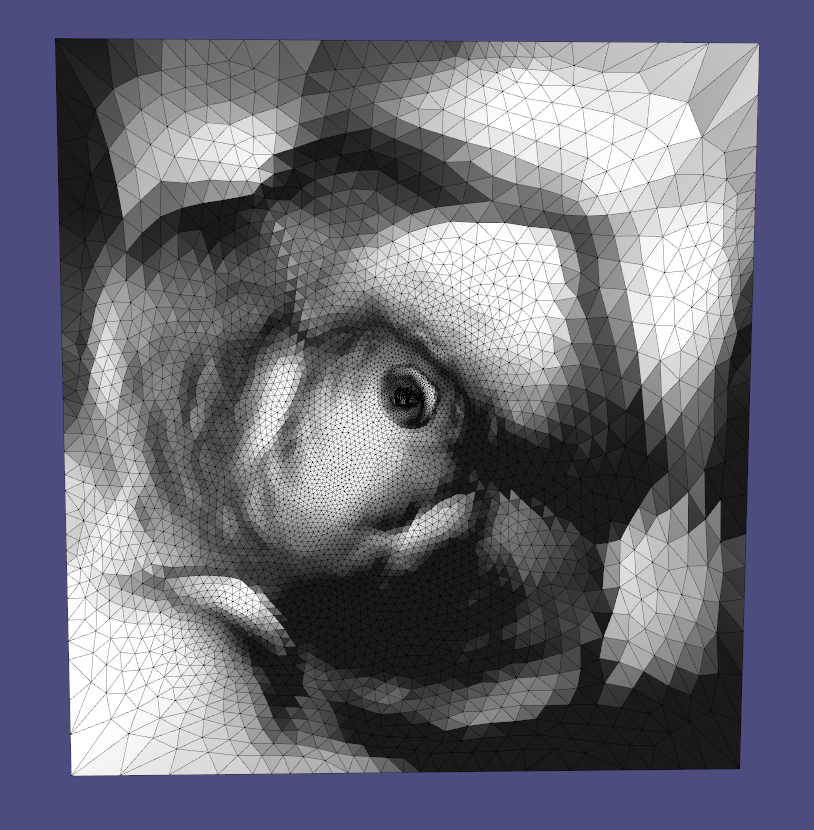
\includegraphics[height = \textwidth]{images/bunny_polygon_emb}
\caption{}
\end{subfigure}\ \ \ \ \ \ \ \ \ 
\begin{subfigure}{0.25\textwidth}
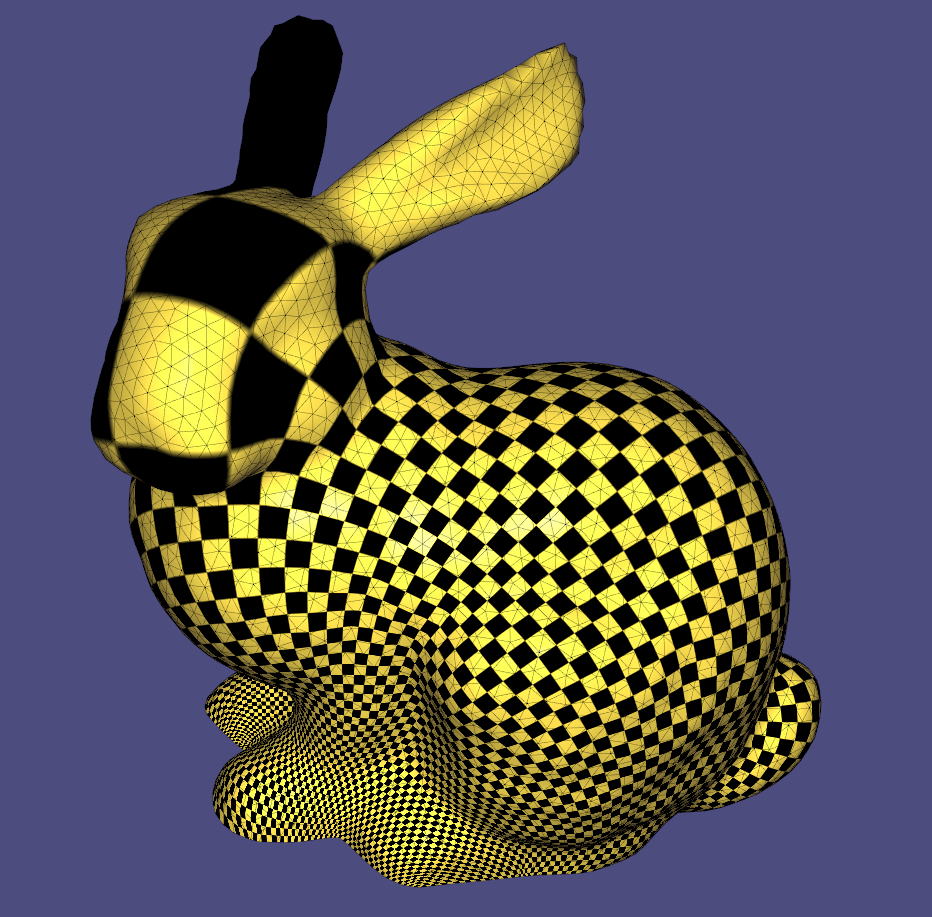
\includegraphics[height = \textwidth]{images/bunny_polygon_texture}
\caption{}
\end{subfigure}

\begin{subfigure}{0.25\textwidth}
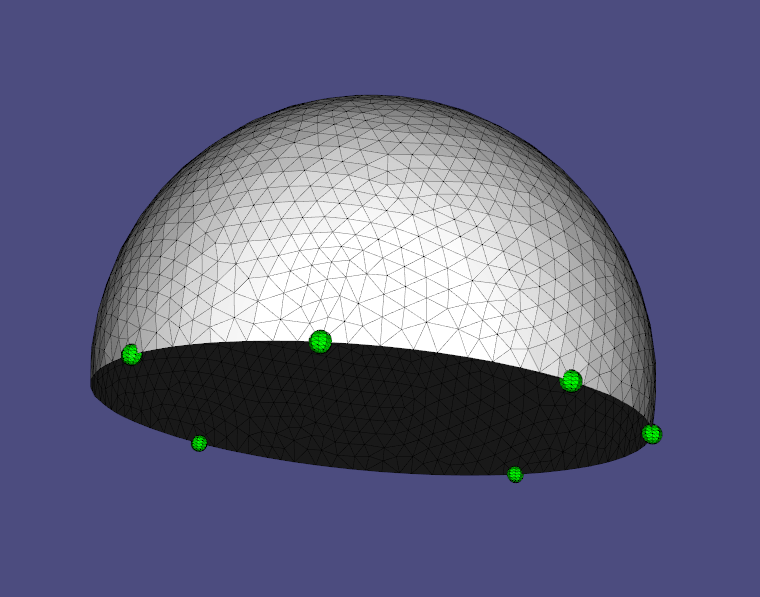
\includegraphics[height = \textwidth]{images/halfshpere_polygon}
\caption{}
\end{subfigure}\ \ \ \ \ \ \ \ \ \ \ \ \
\begin{subfigure}{0.25\textwidth}
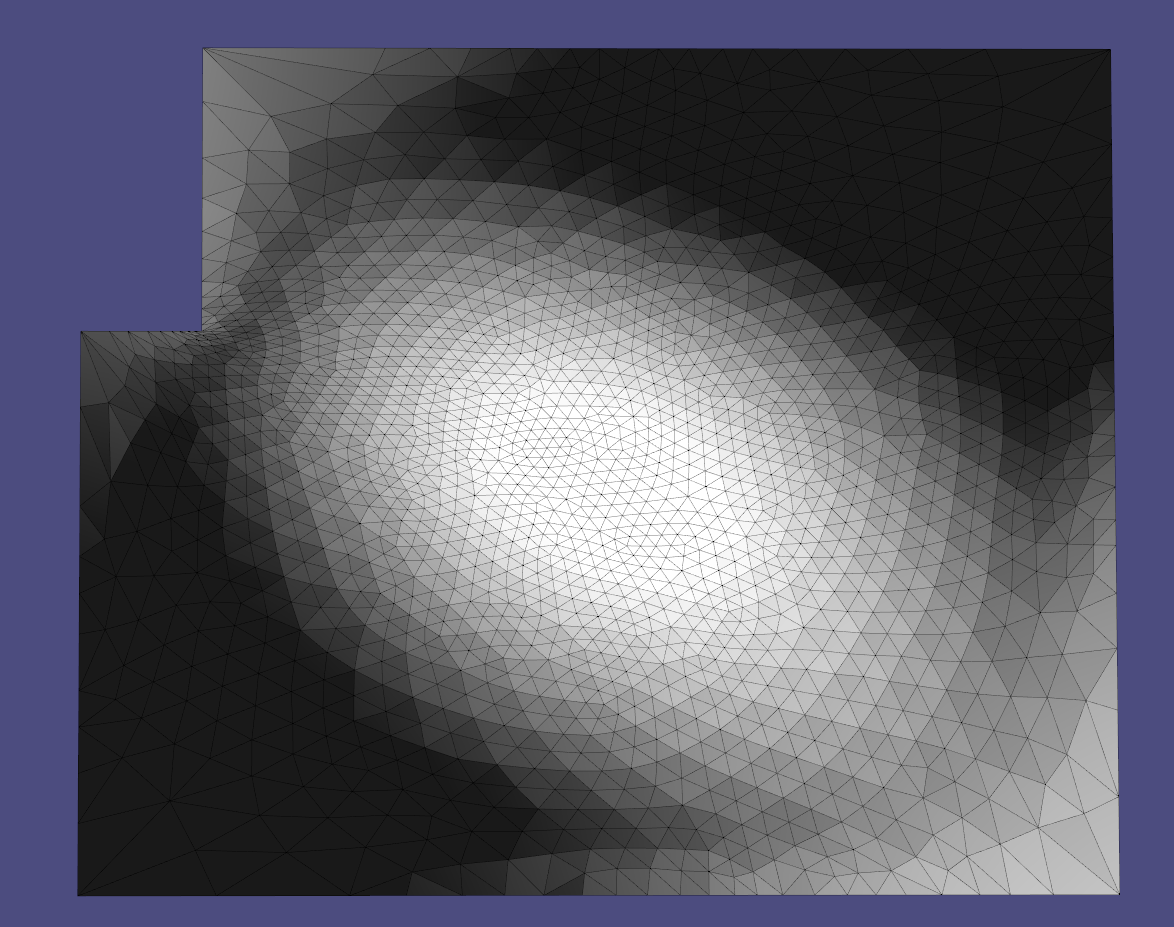
\includegraphics[height = \textwidth]{images/halfsphere_polygon_emb}
\caption{}
\end{subfigure}\ \ \ \ \ \ \ \ \ \ \ \ \
\begin{subfigure}{0.25\textwidth}
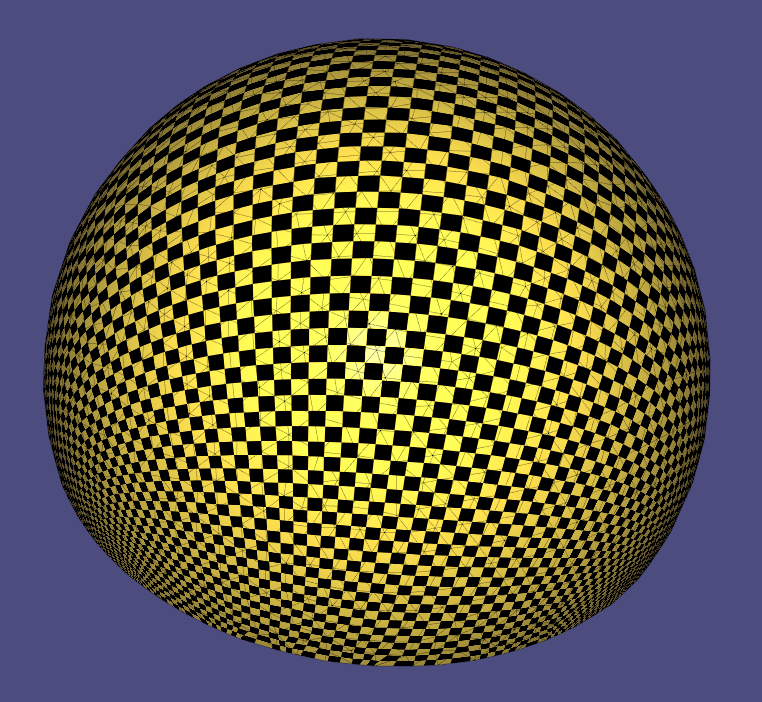
\includegraphics[height = \textwidth]{images/halfshpere_polygon_texture}
\caption{}
\end{subfigure}
\caption{Polygon-boundary conformal maps.(a)(d) Cones. (b)(e) Embedding. (c)(f) Texture mapping.}
\label{fig:polygon}
\end{figure}
Note that we achieve a harmonic map with non-convex boundary. Many algorithms will fail on non convex boundary.


\subsubsection{Cone Parameterization}
A powerful technique for mitigating area distortion is to first map to a cone surface, which is flat (K = 0) away from a collection of isolated cone points.

Known cones and its angles, we first solve the Cherrier problem to get $u$, with source term $\Omega - \tilde{\Omega}$  and boundary data $h = \tilde{k} - k$. Then we feed the $u$ to our algorithm. The result is shown in Fig.\ref{fig:cone}.

\begin{figure}
\centering
\begin{subfigure}{0.25\textwidth}
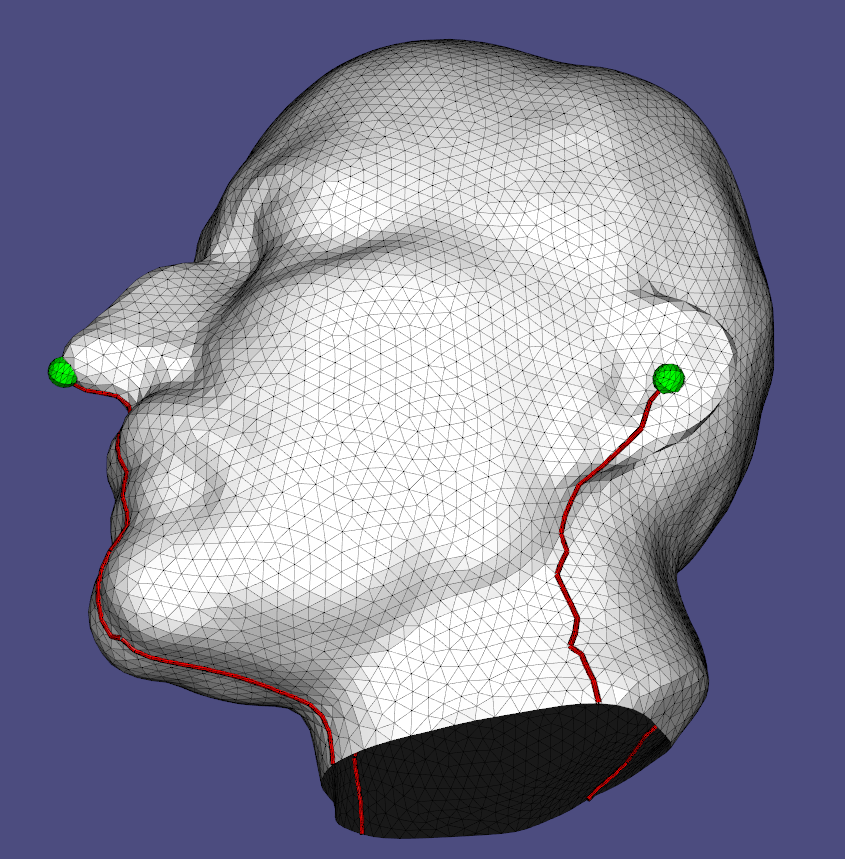
\includegraphics[height = \textwidth]{images/max_global}
\caption{}
\end{subfigure}\ \ \ \ \ \ \ \ \ 
\begin{subfigure}{0.25\textwidth}
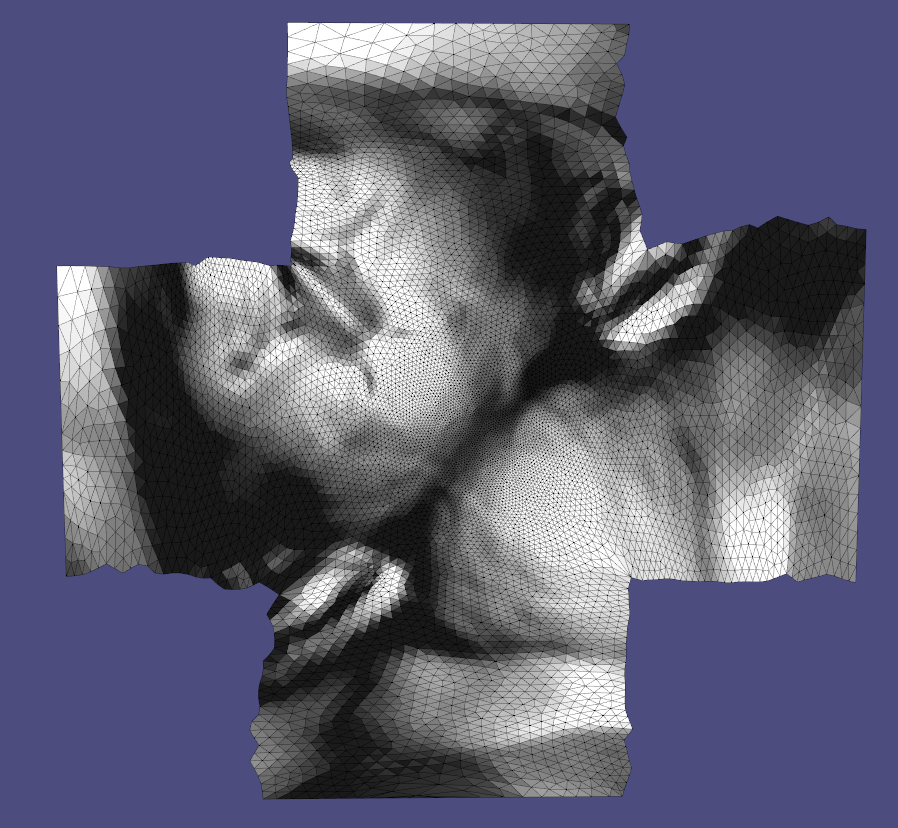
\includegraphics[height = \textwidth]{images/max_global_emb}
\caption{}
\end{subfigure}\ \ \ \ \ \ \ \ \ 
\begin{subfigure}{0.25\textwidth}
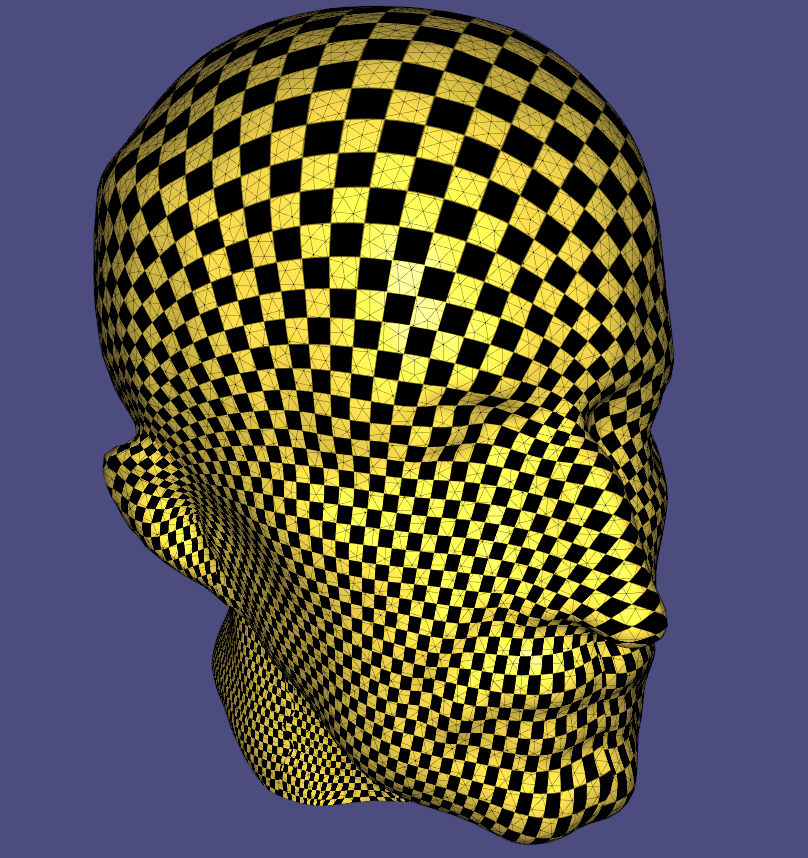
\includegraphics[height = \textwidth]{images/max_global_texture}
\caption{}
\end{subfigure}
\caption{Conformal maps with cones. (a) Cones. (b) Embedding. (c) Texture mapping.}
\label{fig:cone}
\end{figure}












